\begin{defn}{Cone Condition}~\label{def:cone_condition}
    Let $E$ be a Euclidean space and let $G$ be an open subset of $E$.
    Let $\varepsilon >0$, and define 
    $V(w, l)$ to be a cone with vertex at origo, opening $\varepsilon$, axis $w$,
    and height $l$.
    Also define $\mathcal{E} = \{e(g) | g \in G, \, e(g) \text{ is a straight line}\}$ 
    to be the set of all possible straight lines going through each point in $G$. %Kan det misfortåes? Linjen skal ikke gå gennem alle, men et specifikt punkt.
    The cone condition is defined to be:
    \begin{equation*}
        \exists h, 0\leq h \leq \infty \quad
        \exists e\in \mathcal{E} \,\, : \,\,  x \in G \implies 
        x + V(e(x), h) \subset G. % + er translation
    \end{equation*}
    This means: at all points in $G$, we can create a cone with positive opening,
    with some height, pointing in some direction, such that the cone is contained 
    in $G$.
\end{defn}
\begin{figure}[H]
    \center
    \begin{tikzpicture}
	\path[draw=black, line width =1pt, line join=round]  (0,0) .. controls (-0.2,1.5) .. (1,1)
		-- (1.5,1) .. controls (1,0) .. (1.2,-0.2)
		.. controls (1.5,-1.5) .. (-0.25,-1)
		.. controls (-0.5, -0.5) .. cycle;
  \node [isosceles triangle,
         isosceles triangle apex angle=20,
         rotate = 30,
         fill=gray!25,
         anchor=apex,
         minimum width=2pt] (t) at (1.5,1) {};    
\end{tikzpicture}
    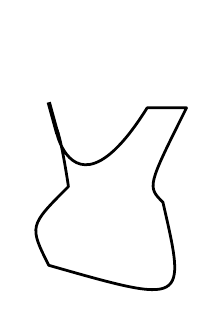
\begin{tikzpicture}
	\path[draw=black, line width =1pt, line join=round]  (0,0) .. controls (-0.3,2) and 
		(-0.25, -1) .. (1,1)
		-- (1.5,1) .. controls (1,0) .. (1.2,-0.2)
		.. controls (1.5,-1.5) .. (-0.25,-1)
		.. controls (-0.5, -0.5) .. cycle;
	\path[draw=black, line width = 1.5pt, line join=round] (-0.14,0.67) -- (-0.25,1.07);
\end{tikzpicture}
\end{figure}
%TODO Anton vil gerne have billeder


%Hovedkilder: https://encyclopediaofmath.org/wiki/Cone#cite_note-Right_circular_cone-1
% https://encyclopediaofmath.org/wiki/Cone_condition